\chapter{Hardware} %Cebrail

During the project we have worked with two Arduino types. Duemilanove and Leonardo clone.
The clone was more powerful and therefore was our main used board. The clone is called
OLIMEXINO-32U4.
\subsection{Specications}

\subsubsection{Arduino}
The specs of the Arduino boards vary very much of each other. The OLIMEXINO is definitely
better.

\begin{table}[h]
\resizebox{16cm}{!} {
    \begin{tabular}{l|l|l|l|l|l|l}
    Board name     & Microcontroller & Operating Voltage & Flash Memory & Clock Speed & Input Power & SRAM   \\ \hline
    OLIMEXINO-32U4 & ATMEGA32U4      & 3.3V / 5V         & 32KB         & 16 MHz      & 7-12VDC     & 2.5 KB \\
    Duemilanove    & ATmega168       & 5V                & 16 KB        & 16 MHz      & 7-12V       & 1 KB   \\
    \end{tabular}
}
    \caption{Specifications of the boards}
\end{table}

\subsubsection{Gameduino2}
The specificatins of the Gameduino2\footnote{http://excamera.com/sphinx/gameduino2/} shield.

\begin{itemize}
  \footnotesize
  \item Video output is 480x272 pixels in 24-bit color.
  \item OpenGL-style command set.
  \item Up to 2000 sprites, any size.
  \item 256 Kbytes of video RAM.
  \item Smooth sprite rotate and zoom with bilinear filtering.
  \item Smooth circle and line drawing in hardware - 16x antialiased.
  \item JPEG loading in hardware.
  \item Built-in rendering of gradients, text, dials and buttons.
\end{itemize}


\subsection{input}
The Wii nunchuk is one of the ways to control the game, aside from the
touchscreen.
The nunchuk has to be connected to the Arduino by hardware. Even though they
use same slots in the board, it is possible to use both the Gameduino 2 and Wii
nunchuk at the same time because they use different hardware interfaces. The
Gameduino uses an ISP interface, while the Wii nunchuk uses an I2C interface.
The Gameduino requires 5 volt to work, which forces us may shorten the lifetime
of the nunchuk - as it normally operates at 3.3 volt, but it should not be a
big concern.


\begin{figure}[h]
\centering
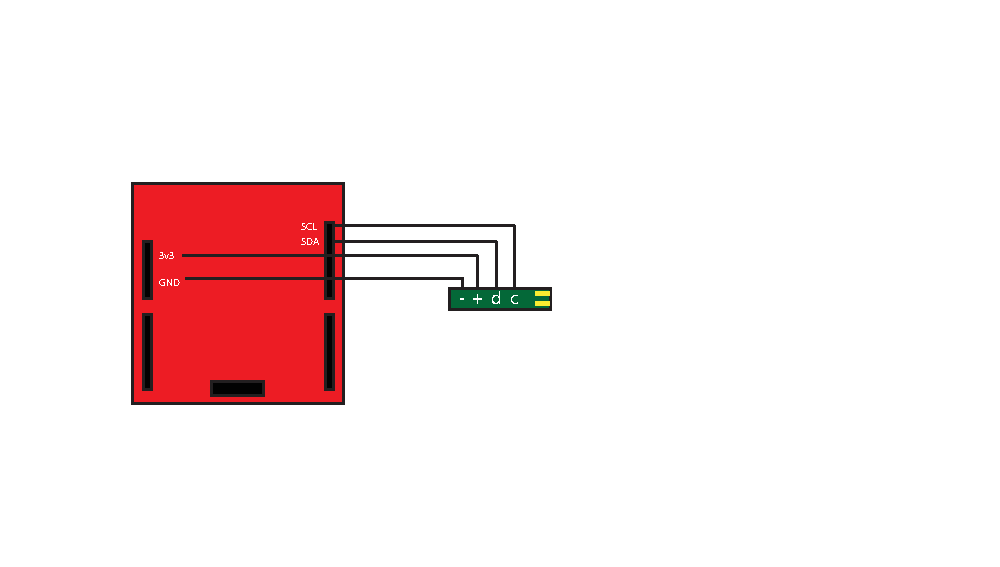
\includegraphics{Figures/NunchuckConnection}
\caption{Hardware connection of an nunchuk}
\label{fig:nunchuk_connect}
\end{figure}


\subsection{I2C}
The I2C is the interface, which is used by the Wii nunchuk adapter. This bus
interface allows easy communication between components and only requires two
bus lines. These lines are both bidirectional. These bus lines are called SCL
(Serial Clock Line) and SDA (Serial Data Line).


\begin{figure}[h]
\centering
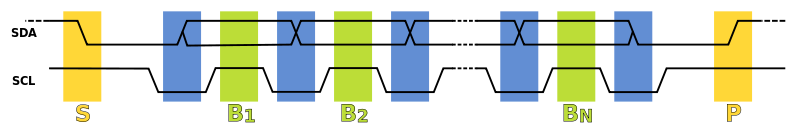
\includegraphics[scale=0.4]{Figures/I2C}
\caption{Hardware connection of an nunchuk}
\label{fig:i2c}
\end{figure}


\begin{enumerate}
\item Data trans fer is initiated with a START bit (S) signaled by SDA being
pulled low while SCL stays high.
\item SDA sets the 1st data bit level while keeping SCL low (during blue bar
time.) and the data is sampled (received) when SCL rises (green).
\item When the transfer is complete, a STOP bit (P) is sent by releasing the
data line to allow it to be pulled high while SCL is kept high continuously.
\item In order to avoid false marker detection, the level on SDA is changed on
the SCL falling edge and is sampled and captured on the rising edge of SCL.
\end{enumerate}








